%\documentclass[11pt,a4paper]{article}
%\usepackage[utf8]{inputenc}
%\usepackage{amsmath}
%\usepackage{amsfonts}
%\usepackage{amssymb}
%\usepackage{graphicx}
%\usepackage{color}
%\usepackage{caption}
%\usepackage{wrapfig}
%\usepackage{textcomp}
%\usepackage[left=2.5cm,right=2.5cm,top=2.5cm,bottom=2.5cm]{geometry}
%\usepackage{mathtools, bm}
%\usepackage{amssymb, bm}
%\usepackage{fancyhdr}
%\usepackage{fancybox}
%\usepackage{listings}


\documentclass[11pt,fleqn]{book} % Default font size and left-justified equations

%----------------------------------------------------------------------------------------

%%%%%%%%%%%%%%%%%%%%%%%%%%%%%%%%%%%%%%%%%
% The Legrand Orange Book
% Structural Definitions File
% Version 2.0 (9/2/15)
%
% Original author:
% Mathias Legrand (legrand.mathias@gmail.com) with modifications by:
% Vel (vel@latextemplates.com)
% 
% This file has been downloaded from:
% http://www.LaTeXTemplates.com
%
% License:
% CC BY-NC-SA 3.0 (http://creativecommons.org/licenses/by-nc-sa/3.0/)
%
%%%%%%%%%%%%%%%%%%%%%%%%%%%%%%%%%%%%%%%%%

%----------------------------------------------------------------------------------------
%	VARIOUS REQUIRED PACKAGES AND CONFIGURATIONS
%----------------------------------------------------------------------------------------

\usepackage[top=3cm,bottom=3cm,left=3cm,right=3cm,headsep=10pt,a4paper]{geometry} % Page margins

\usepackage{graphicx} % Required for including pictures
\graphicspath{{Pictures/}} % Specifies the directory where pictures are stored

\usepackage{tikz} % Required for drawing custom shapes

\usepackage[francais]{babel} % English language/hyphenation

\usepackage{enumitem} % Customize lists
\setlist{nolistsep} % Reduce spacing between bullet points and numbered lists

\usepackage{booktabs} % Required for nicer horizontal rules in tables

\usepackage{xcolor} % Required for specifying colors by name
\definecolor{ocre}{RGB}{43,102,25} % Define the orange color used for highlighting throughout the book

\usepackage{listings}
\usepackage{ccaption}
%----------------------------------------------------------------------------------------
%	FONTS
%----------------------------------------------------------------------------------------

\usepackage{avant} % Use the Avantgarde font for headings
%\usepackage{times} % Use the Times font for headings
\usepackage{mathptmx} % Use the Adobe Times Roman as the default text font together with math symbols from the Sym­bol, Chancery and Com­puter Modern fonts

\usepackage{microtype} % Slightly tweak font spacing for aesthetics
\usepackage[utf8]{inputenc} % Required for including letters with accents
\usepackage[T1]{fontenc} % Use 8-bit encoding that has 256 glyphs

%----------------------------------------------------------------------------------------
%	BIBLIOGRAPHY AND INDEX
%----------------------------------------------------------------------------------------

\usepackage[style=alphabetic,citestyle=numeric,sorting=nyt,sortcites=true,autopunct=true,babel=hyphen,hyperref=true,abbreviate=false,backref=true,backend=biber]{biblatex}
\addbibresource{bibliography.bib} % BibTeX bibliography file
\defbibheading{bibempty}{}

\usepackage{calc} % For simpler calculation - used for spacing the index letter headings correctly
\usepackage{makeidx} % Required to make an index
\makeindex % Tells LaTeX to create the files required for indexing

%----------------------------------------------------------------------------------------
%	MAIN TABLE OF CONTENTS
%----------------------------------------------------------------------------------------

\usepackage{titletoc} % Required for manipulating the table of contents

\contentsmargin{0cm} % Removes the default margin

% Part text styling
\titlecontents{part}[0cm]
{\addvspace{20pt}\centering\large\bfseries}
{}
{}
{}

% Chapter text styling
\titlecontents{chapter}[1.25cm] % Indentation
{\addvspace{12pt}\large\sffamily\bfseries} % Spacing and font options for chapters
{\color{ocre!60}\contentslabel[\Large\thecontentslabel]{1.25cm}\color{ocre}} % Chapter number
{\color{ocre}}  
{\color{ocre!60}\normalsize\;\titlerule*[.5pc]{.}\;\thecontentspage} % Page number

% Section text styling
\titlecontents{section}[1.25cm] % Indentation
{\addvspace{3pt}\sffamily\bfseries} % Spacing and font options for sections
{\contentslabel[\thecontentslabel]{1.25cm}} % Section number
{}
{\hfill\color{black}\thecontentspage} % Page number
[]

% Subsection text styling
\titlecontents{subsection}[1.25cm] % Indentation
{\addvspace{1pt}\sffamily\small} % Spacing and font options for subsections
{\contentslabel[\thecontentslabel]{1.25cm}} % Subsection number
{}
{\ \titlerule*[.5pc]{.}\;\thecontentspage} % Page number
[]

% List of figures
\titlecontents{figure}[0em]
{\addvspace{-5pt}\sffamily}
{\thecontentslabel\hspace*{1em}}
{}
{\ \titlerule*[.5pc]{.}\;\thecontentspage}
[]

% List of tables
\titlecontents{table}[0em]
{\addvspace{-5pt}\sffamily}
{\thecontentslabel\hspace*{1em}}
{}
{\ \titlerule*[.5pc]{.}\;\thecontentspage}
[]

%----------------------------------------------------------------------------------------
%	MINI TABLE OF CONTENTS IN PART HEADS
%----------------------------------------------------------------------------------------

% Chapter text styling
\titlecontents{lchapter}[0em] % Indenting
{\addvspace{15pt}\large\sffamily\bfseries} % Spacing and font options for chapters
{\color{ocre}\contentslabel[\Large\thecontentslabel]{1.25cm}\color{ocre}} % Chapter number
{}  
{\color{ocre}\normalsize\sffamily\bfseries\;\titlerule*[.5pc]{.}\;\thecontentspage} % Page number

% Section text styling
\titlecontents{lsection}[0em] % Indenting
{\sffamily\small} % Spacing and font options for sections
{\contentslabel[\thecontentslabel]{1.25cm}} % Section number
{}
{}

% Subsection text styling
\titlecontents{lsubsection}[.5em] % Indentation
{\normalfont\footnotesize\sffamily} % Font settings
{}
{}
{}

%----------------------------------------------------------------------------------------
%	PAGE HEADERS
%----------------------------------------------------------------------------------------

\usepackage{fancyhdr} % Required for header and footer configuration

\pagestyle{fancy}
\renewcommand{\chaptermark}[1]{\markboth{\sffamily\normalsize\bfseries\chaptername\ \thechapter.\ #1}{}} % Chapter text font settings
\renewcommand{\sectionmark}[1]{\markright{\sffamily\normalsize\thesection\hspace{5pt}#1}{}} % Section text font settings
\fancyhf{} \fancyfoot[LE,RO]{\sffamily\normalsize\thepage} % Font setting for the page number in the header
%\fancyhead[LO]{\rightmark} % Print the nearest section name on the left side of odd pages
%\fancyhead[RE]{\leftmark} % Print the current chapter name on the right side of even pages
\fancyhead[L]{Lycée Rouvière / PB}
\fancyhead[R]{PTSI / Informatique / DS2}
\renewcommand{\headrulewidth}{0.5pt} % Width of the rule under the header
\addtolength{\headheight}{2.5pt} % Increase the spacing around the header slightly
\renewcommand{\footrulewidth}{0pt} % Removes the rule in the footer
\fancypagestyle{plain}{\fancyhead{}\renewcommand{\headrulewidth}{0pt}} % Style for when a plain pagestyle is specified

% Removes the header from odd empty pages at the end of chapters
%\makeatletter
%\renewcommand{\cleardoublepage}{
%\clearpage\ifodd\c@page\else
%\hbox{}
%\vspace*{\fill}
%\thispagestyle{empty}
%\newpage
%\fi}

%----------------------------------------------------------------------------------------
%	THEOREM STYLES
%----------------------------------------------------------------------------------------

\usepackage{amsmath,amsfonts,amssymb,amsthm} % For math equations, theorems, symbols, etc

\newcommand{\intoo}[2]{\mathopen{]}#1\,;#2\mathclose{[}}
\newcommand{\ud}{\mathop{\mathrm{{}d}}\mathopen{}}
\newcommand{\intff}[2]{\mathopen{[}#1\,;#2\mathclose{]}}
\newtheorem{notation}{Notation}[chapter]

% Boxed/framed environments
\newtheoremstyle{ocrenumbox}% % Theorem style name
{0pt}% Space above
{0pt}% Space below
{\normalfont}% % Body font
{}% Indent amount
{\small\bf\sffamily\color{ocre}}% % Theorem head font
{\;}% Punctuation after theorem head
{0.25em}% Space after theorem head
{\small\sffamily\color{ocre}\thmname{#1}\nobreakspace
{\@ifnotempty{#1}{}\@upn{#2}}% Theorem text (e.g. Theorem 2.1)
\thmnote{\nobreakspace\the\thm@notefont\sffamily\bfseries\color{black}---\nobreakspace#3.}} % Optional theorem note
\renewcommand{\qedsymbol}{$\blacksquare$}% Optional qed square

\newtheoremstyle{blacknumex}% Theorem style name
{5pt}% Space above
{5pt}% Space below
{\normalfont}% Body font
{} % Indent amount
{\small\bf\sffamily}% Theorem head font
{\;}% Punctuation after theorem head
{0.25em}% Space after theorem head
{\small\sffamily{\tiny\ensuremath{\blacksquare}}\nobreakspace\thmname{#1}\nobreakspace{\@ifnotempty{#1}{}\@upn{#2}}% Theorem text (e.g. Theorem 2.1)
\thmnote{\nobreakspace\the\thm@notefont\sffamily\bfseries---\nobreakspace#3.}}% Optional theorem note

\newtheoremstyle{blacknumbox} % Theorem style name
{0pt}% Space above
{0pt}% Space below
{\normalfont}% Body font
{}% Indent amount
{\small\bf\sffamily}% Theorem head font
{\;}% Punctuation after theorem head
{0.25em}% Space after theorem head
{\small\sffamily\thmname{#1}\nobreakspace{\@ifnotempty{#1}{}\@upn{#2}}% Theorem text (e.g. Theorem 2.1)
\thmnote{\nobreakspace\the\thm@notefont\sffamily\bfseries---\nobreakspace#3.}}% Optional theorem note

% Non-boxed/non-framed environments
\newtheoremstyle{ocrenum}% % Theorem style name
{5pt}% Space above
{5pt}% Space below
{\normalfont}% % Body font
{}% Indent amount
{\small\bf\sffamily\color{ocre}}% % Theorem head font
{\;}% Punctuation after theorem head
{0.25em}% Space after theorem head
{\small\sffamily\color{ocre}\thmname{#1}\nobreakspace
{\@ifnotempty{#1}{}\@upn{#2}}% Theorem text (e.g. Theorem 2.1)
\thmnote{\nobreakspace\the\thm@notefont\sffamily\bfseries\color{black}---\nobreakspace#3.}} % Optional theorem note
\renewcommand{\qedsymbol}{$\blacksquare$}% Optional qed square
\makeatother

% Defines the theorem text style for each type of theorem to one of the three styles above
\newcounter{dummy} 
\numberwithin{dummy}{section}
\theoremstyle{ocrenumbox}
\newtheorem{theoremeT}[dummy]{Theorem}
\newtheorem{problem}{Problem}[chapter]
\newtheorem{exerciseT}{Exercise}[chapter]
\theoremstyle{blacknumex}
\newtheorem{exampleT}{Example}[chapter]
\theoremstyle{blacknumbox}
\newtheorem{vocabulary}{Vocabulary}[chapter]
\newtheorem{definitionT}{}[]
\newtheorem{corollaryT}[dummy]{Corollary}
\theoremstyle{ocrenum}
\newtheorem{proposition}[dummy]{Proposition}

%----------------------------------------------------------------------------------------
%	DEFINITION OF COLORED BOXES
%----------------------------------------------------------------------------------------

\RequirePackage[framemethod=default]{mdframed} % Required for creating the theorem, definition, exercise and corollary boxes

% Theorem box
\newmdenv[skipabove=7pt,
skipbelow=7pt,
backgroundcolor=black!5,
linecolor=ocre,
innerleftmargin=5pt,
innerrightmargin=5pt,
innertopmargin=5pt,
leftmargin=0cm,
rightmargin=0cm,
innerbottommargin=5pt]{tBox}

% Exercise box	  
\newmdenv[skipabove=7pt,
skipbelow=7pt,
rightline=false,
leftline=true,
topline=false,
bottomline=false,
backgroundcolor=ocre!10,
linecolor=ocre,
innerleftmargin=5pt,
innerrightmargin=5pt,
innertopmargin=5pt,
innerbottommargin=5pt,
leftmargin=0cm,
rightmargin=0cm,
linewidth=4pt]{eBox}	

% Definition box
\newmdenv[skipabove=7pt,
skipbelow=7pt,
rightline=false,
leftline=true,
topline=false,
bottomline=false,
linecolor=ocre,
innerleftmargin=5pt,
innerrightmargin=5pt,
innertopmargin=0pt,
leftmargin=0cm,
rightmargin=0cm,
linewidth=4pt,
innerbottommargin=0pt]{dBox}	

% Corollary box
\newmdenv[skipabove=7pt,
skipbelow=7pt,
rightline=false,
leftline=true,
topline=false,
bottomline=false,
linecolor=gray,
backgroundcolor=black!5,
innerleftmargin=5pt,
innerrightmargin=5pt,
innertopmargin=5pt,
leftmargin=0cm,
rightmargin=0cm,
linewidth=4pt,
innerbottommargin=5pt]{cBox}

% Creates an environment for each type of theorem and assigns it a theorem text style from the "Theorem Styles" section above and a colored box from above
\newenvironment{theorem}{\begin{tBox}\begin{theoremeT}}{\end{theoremeT}\end{tBox}}
\newenvironment{exercise}{\begin{eBox}\begin{exerciseT}}{\hfill{\color{ocre}\tiny\ensuremath{\blacksquare}}\end{exerciseT}\end{eBox}}				  
\newenvironment{definition}{\begin{dBox}\begin{definitionT}}{\end{definitionT}\end{dBox}}

\newenvironment{example}{\begin{exampleT}}{\hfill{\tiny\ensuremath{\blacksquare}}\end{exampleT}}		
\newenvironment{corollary}{\begin{cBox}\begin{corollaryT}}{\end{corollaryT}\end{cBox}}	

%----------------------------------------------------------------------------------------
%	REMARK ENVIRONMENT
%----------------------------------------------------------------------------------------

\newenvironment{remark}{\par\vspace{10pt}\small % Vertical white space above the remark and smaller font size
\begin{list}{}{
\leftmargin=35pt % Indentation on the left
\rightmargin=25pt}\item\ignorespaces % Indentation on the right
\makebox[-2.5pt]{\begin{tikzpicture}[overlay]
\node[draw=ocre!60,line width=1pt,circle,fill=ocre!25,font=\sffamily\bfseries,inner sep=2pt,outer sep=0pt] at (-15pt,0pt){\textcolor{ocre}{R}};\end{tikzpicture}} % Orange R in a circle
\advance\baselineskip -1pt}{\end{list}\vskip5pt} % Tighter line spacing and white space after remark

%----------------------------------------------------------------------------------------
%	SECTION NUMBERING IN THE MARGIN
%----------------------------------------------------------------------------------------

\makeatletter
\renewcommand{\@seccntformat}[1]{\llap{\textcolor{ocre}{\csname the#1\endcsname}\hspace{1em}}}                   
\renewcommand{\section}{\@startsection{section}{1}{\z@}
{-4ex \@plus -1ex \@minus -.4ex}
{1ex \@plus.2ex }
{\normalfont\large\sffamily\bfseries}}
\renewcommand{\subsection}{\@startsection {subsection}{2}{\z@}
{-3ex \@plus -0.1ex \@minus -.4ex}
{0.5ex \@plus.2ex }
{\normalfont\sffamily\bfseries}}
\renewcommand{\subsubsection}{\@startsection {subsubsection}{3}{\z@}
{-2ex \@plus -0.1ex \@minus -.2ex}
{.2ex \@plus.2ex }
{\normalfont\small\sffamily\bfseries}}                        
\renewcommand\paragraph{\@startsection{paragraph}{4}{\z@}
{-2ex \@plus-.2ex \@minus .2ex}
{.1ex}
{\normalfont\small\sffamily\bfseries}}

%----------------------------------------------------------------------------------------
%	PART HEADINGS
%----------------------------------------------------------------------------------------

% numbered part in the table of contents
\newcommand{\@mypartnumtocformat}[2]{%
\setlength\fboxsep{0pt}%
\noindent\colorbox{ocre!20}{\strut\parbox[c][.7cm]{\ecart}{\color{ocre!70}\Large\sffamily\bfseries\centering#1}}\hskip\esp\colorbox{ocre!40}{\strut\parbox[c][.7cm]{\linewidth-\ecart-\esp}{\Large\sffamily\centering#2}}}%
%%%%%%%%%%%%%%%%%%%%%%%%%%%%%%%%%%
% unnumbered part in the table of contents
\newcommand{\@myparttocformat}[1]{%
\setlength\fboxsep{0pt}%
\noindent\colorbox{ocre!40}{\strut\parbox[c][.7cm]{\linewidth}{\Large\sffamily\centering#1}}}%
%%%%%%%%%%%%%%%%%%%%%%%%%%%%%%%%%%
\newlength\esp
\setlength\esp{4pt}
\newlength\ecart
\setlength\ecart{1.2cm-\esp}
\newcommand{\thepartimage}{}%
\newcommand{\partimage}[1]{\renewcommand{\thepartimage}{#1}}%
\def\@part[#1]#2{%
\ifnum \c@secnumdepth >-2\relax%
\refstepcounter{part}%
\addcontentsline{toc}{part}{\texorpdfstring{\protect\@mypartnumtocformat{\thepart}{#1}}{\partname~\thepart\ ---\ #1}}
\else%
\addcontentsline{toc}{part}{\texorpdfstring{\protect\@myparttocformat{#1}}{#1}}%
\fi%
\startcontents%
\markboth{}{}%
{\thispagestyle{empty}%
\begin{tikzpicture}[remember picture,overlay]%
\node at (current page.north west){\begin{tikzpicture}[remember picture,overlay]%	
\fill[ocre!20](0cm,0cm) rectangle (\paperwidth,-\paperheight);
\node[anchor=north] at (4cm,-3.25cm){\color{ocre!40}\fontsize{220}{100}\sffamily\bfseries\@Roman\c@part}; 
\node[anchor=south east] at (\paperwidth-1cm,-\paperheight+1cm){\parbox[t][][t]{8.5cm}{
\printcontents{l}{0}{\setcounter{tocdepth}{1}}%
}};
\node[anchor=north east] at (\paperwidth-1.5cm,-3.25cm){\parbox[t][][t]{15cm}{\strut\raggedleft\color{white}\fontsize{30}{30}\sffamily\bfseries#2}};
\end{tikzpicture}};
\end{tikzpicture}}%
\@endpart}
\def\@spart#1{%
\startcontents%
\phantomsection
{\thispagestyle{empty}%
\begin{tikzpicture}[remember picture,overlay]%
\node at (current page.north west){\begin{tikzpicture}[remember picture,overlay]%	
\fill[ocre!20](0cm,0cm) rectangle (\paperwidth,-\paperheight);
\node[anchor=north east] at (\paperwidth-1.5cm,-3.25cm){\parbox[t][][t]{22cm}{\strut\raggedleft\color{white}\fontsize{30}{30}\sffamily\bfseries#1}};
\end{tikzpicture}};
\end{tikzpicture}}
\addcontentsline{toc}{part}{\texorpdfstring{%
\setlength\fboxsep{0pt}%
\noindent\protect\colorbox{ocre!40}{\strut\protect\parbox[c][.7cm]{\linewidth}{\Large\sffamily\protect\centering #1\quad\mbox{}}}}{#1}}%
\@endpart}
\def\@endpart{\vfil\newpage
\if@twoside
\if@openright
\null
\thispagestyle{empty}%
\newpage
\fi
\fi
\if@tempswa
\twocolumn
\fi}

%----------------------------------------------------------------------------------------
%	CHAPTER HEADINGS
%----------------------------------------------------------------------------------------

\newcommand{\thechapterimage}{}%
\newcommand{\chapterimage}[1]{\renewcommand{\thechapterimage}{#1}}%
\def\@makechapterhead#1{%
{\parindent \z@ \raggedright \normalfont
\ifnum \c@secnumdepth >\m@ne
\if@mainmatter
\begin{tikzpicture}[remember picture,overlay]
\node at (current page.north west)
{\begin{tikzpicture}[remember picture,overlay]
\node[anchor=north west,inner sep=0pt] at (0,0) {\includegraphics[width=\paperwidth]{\thechapterimage}};
\draw[anchor=west] (\Gm@lmargin,-3cm) node [line width=2pt,rounded corners=15pt,draw=ocre,fill=white,fill opacity=0.5,inner sep=15pt]{\strut\makebox[22cm]{}};
\draw[anchor=west] (\Gm@lmargin+.3cm,-3cm) node {\huge\sffamily\bfseries\color{black} #1\strut};
\end{tikzpicture}};
\end{tikzpicture}
\else
\begin{tikzpicture}[remember picture,overlay]
\node at (current page.north west)
{\begin{tikzpicture}[remember picture,overlay]
\node[anchor=north west,inner sep=0pt] at (0,0) {\includegraphics[width=\paperwidth]{\thechapterimage}};
\draw[anchor=west] (\Gm@lmargin,-3cm) node [line width=2pt,rounded corners=15pt,draw=ocre,fill=white,fill opacity=0.5,inner sep=15pt]{\strut\makebox[22cm]{}};
\draw[anchor=west] (\Gm@lmargin+.3cm,-3cm) node {\huge\sffamily\bfseries\color{black}#1\strut};
\end{tikzpicture}};
\end{tikzpicture}
\fi\fi\par\vspace*{20\p@}}}

%-------------------------------------------

\def\@makeschapterhead#1{%
\begin{tikzpicture}[remember picture,overlay]
\node at (current page.north west)
{\begin{tikzpicture}[remember picture,overlay]
\node[anchor=north west,inner sep=0pt] at (0,0) {\includegraphics[width=\paperwidth]{\thechapterimage}};
\draw[anchor=west] (\Gm@lmargin,-3cm) node [line width=2pt,rounded corners=15pt,draw=ocre,fill=white,fill opacity=0.5,inner sep=15pt]{\strut\makebox[22cm]{}};
\draw[anchor=west] (\Gm@lmargin+.3cm,-3cm) node {\huge\sffamily\bfseries\color{black}#1\strut};
\end{tikzpicture}};
\end{tikzpicture}
\par\vspace*{20\p@}}
\makeatother

%----------------------------------------------------------------------------------------
%	HYPERLINKS IN THE DOCUMENTS
%----------------------------------------------------------------------------------------

\usepackage{hyperref}
\hypersetup{hidelinks,backref=true,pagebackref=true,hyperindex=true,colorlinks=false,breaklinks=true,urlcolor= ocre,bookmarks=true,bookmarksopen=false,pdftitle={Title},pdfauthor={Author}}
\usepackage{bookmark}
\bookmarksetup{
open,
numbered,
addtohook={%
\ifnum\bookmarkget{level}=0 % chapter
\bookmarksetup{bold}%
\fi
\ifnum\bookmarkget{level}=-1 % part
\bookmarksetup{color=ocre,bold}%
\fi
}
}


%\pagestyle{fancy}
%\fancyhead[L]{Lycée Dumont d'Urville / PB}
%\fancyhead[R]{PSI / Informatique / TP}
%\fancyfoot[C]{page \thepage}
%
%\newcommand{\cadretitre}[2]{\boxput*(0,1){
%\colorbox {white}{#1}}{
%\setlength{\fboxsep}{6pt}
%\fbox {\begin{minipage}{\textwidth -0.7cm}
%\bigskip
%#2
%\bigskip
%\end{minipage}}
%}}

\makeatletter
\renewcommand{\thesection}{\@arabic\c@section}
\makeatother

\begin{document}

\chapterimage{image.jpg}
\chapter{PTSI / Informatique / DS \No 2 - 2 h}

\begin{center}
\huge{Analyse harmonique}
\end{center}

\section{Introduction}

L'analyse harmonique (fréquentielle) des systèmes permet de mettre en évidence de nombreuses caractéristiques telles que la bande passante, la fréquence de coupure, la résonance, etc.
Elle sera aussi très utile pour étudier la stabilité d'un système en 2\up{nde} année.

Un système modélisé linéaire peut se caractériser dans le domaine symbolique de Laplace par sa fonction de transfert $H(p)$. Sa forme générale est :

$H(p) = \frac{{{a_m}{p^m} + ... + {a_1}p + {a_0}}}{{{b_n}{p^n} + ... + {b_1}p + {b_0}}}$ où les coefficients $a_i, i \in [0;m]$ et $b_j, j \in [0;n]$ sont réels.

La variable $p$ est un nombre complexe. Pour l'analyse fréquentielle, on pose $p=j \omega$. C'est le cas particulier de la transformée de Fourier. On parle alors aussi de transmittance $H(j \omega)$.

Une représentation classique de cette fonction, est le diagramme de Bode (figure 1). Il fait apparaître deux quantités : le gain (dB) et la phase (\degres).

\begin{figure}[!h]
\begin{center}
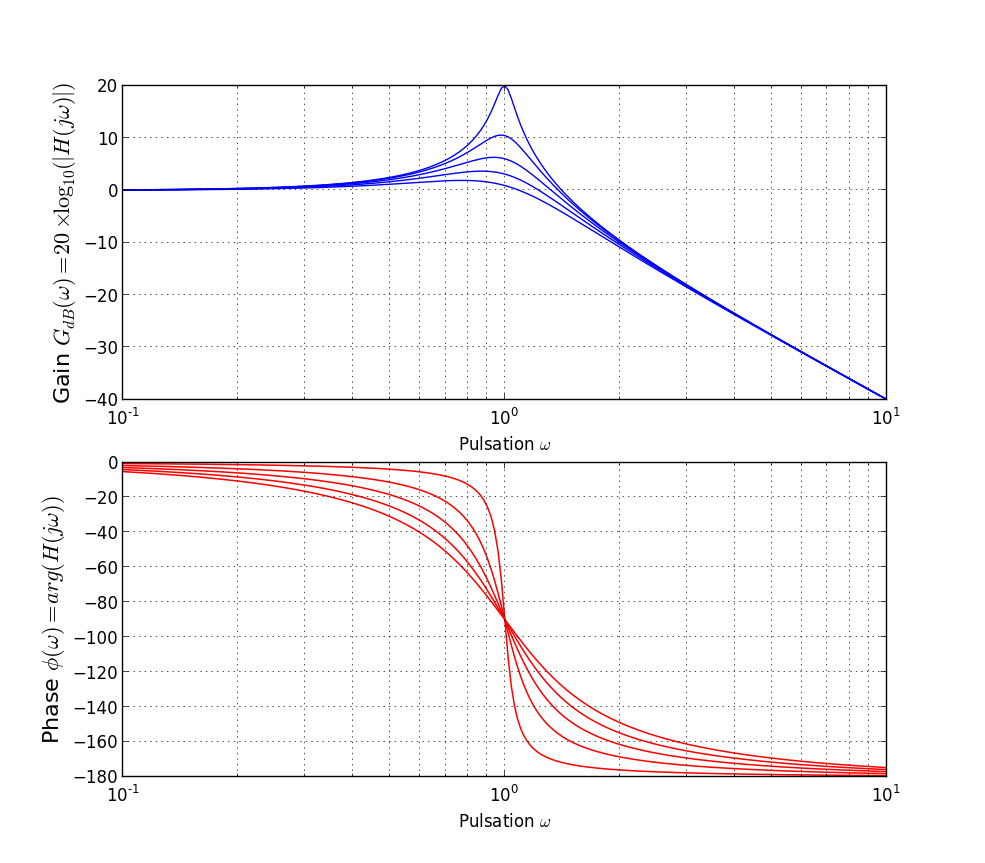
\includegraphics[scale=0.4]{figure_1.png} 
\end{center}
\legend {Fig. 1 : Diagrammes de Bode de systèmes du 2\up{nd} ordre}
\end{figure}

\begin{dBox}
\textit{L'objectif des questions qui suivent est d'extraire certaines propriétés d'un système linéaire à partir de sa fonction de transfert.}
\end{dBox}

\section{Diagramme de Bode}

Le tracé de la figure 1 a été obtenu à l'aide du script donné en annexe 1.

\begin{tBox}
\textbf{Question 1.} Quelles sont les fonctions de transfert dont le diagramme de Bode est représenté sur la figure 1 ?
\end{tBox}

\begin{tBox}
\textbf{Question 2.} A une étape de l'algorithme proposé, 
\begin{enumerate}
\item combien de données contiennent les listes \texttt{w}, \texttt{gain} et \texttt{phase} ?
\item en admettant que chacune de ces données est de type \texttt{float} codé en double précision, quelle quantité de mémoire est nécessaire pour le stockage de ces trois listes ?
\end{enumerate}

\end{tBox}


\section{Propriétés caractéristiques du système}

\subsection{Asymptote infinie de la courbe en gain}

Trois listes de même dimension \texttt{w}, \texttt{gain} et \texttt{phase} contiennent les données permettant le tracé.
On souhaite déterminer l'asymptote lorsque $\omega \to \infty$ de la courbe de gain de la figure 1. 

\begin{tBox}
\textbf{Question 3.} Proposer un script permettant de donner la valeur de l'asymptote lorsque $\omega \to \infty$ de la courbe de gain en $dB/decade$ (décibels par décade).
\end{tBox}

\subsection{Résonance}

Les courbes en gain de la figure 1 présentent un maximum appelé "pic de résonance". En effet, lorsque le gain est positif, c'est qu'il y a amplification du signal d'entrée.

\begin{tBox}
\textbf{Question 4.} Dans le contexte de la figure 1, écrire la fonction \texttt{picResonance(w,gain,phase)} retournant pour une courbe un triplet de valeurs respectives la pulsation de résonance $wr$, le gain maximal $gr$ et la phase correspondante $pr$ :\texttt{(wr,gr,pr)}. Dans le cas où ce pic n'existerait pas, elle retourne un triplet vide.
\end{tBox}

Dans certains cas, le système peut présenter plusieurs pics de résonance (figure 2).

\begin{figure}[!h]
\begin{center}
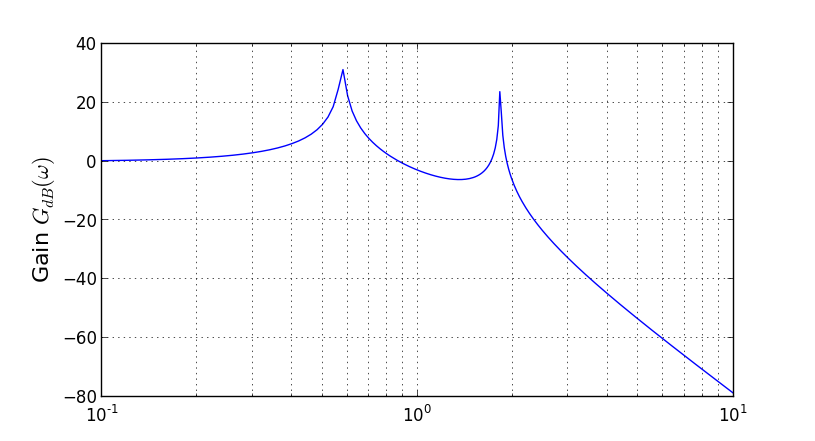
\includegraphics[scale=0.5]{figure_2.png} 
\end{center}
\legend {Fig. 2 : Système multi-pics}
\end{figure}

\begin{tBox}
\textbf{Question 5.} Dans le cas où le diagramme en gain serait multi-pics, écrire la fonction \\ \texttt{picsResonance(w,gain,phase)} retournant une liste \texttt{L} de triplets de valeurs respectives une pulsation de résonance $wr$, le gain $gr$ et la phase correspondante $pr$ :\texttt{(wr,gr,pr)}. La liste \texttt{L} peut présenter l'allure suivante : \texttt{[(wr1,gr1,pr1),(wr2,gr2,pr2),...,(wrk,grk,prk)]}. Dans le cas où il n'y aurait aucun pics, la fonction retourne une liste vide.
\end{tBox}


\pagebreak

\subsection{Bande passante}

\begin{dBox}
Pour un filtre passe-bas, la bande passante peut être définie comme la plage de pulsations $\omega \in ]0;\omega_c]$ pour lesquelles le gain est supérieur ou égal à $G_{max}-3 dB$. On peut ainsi préciser la pulsation de coupure $\omega_c$.
\end{dBox}



Dans tout ce qui suit, on se place dans le cas d'un filtre passe-bas passif ($G_{dB}(0) = 0)$ non résonant. La fonction $G_{dB}$ est monotone décroissante et l'équation $G_{dB}(\omega) + 3 = 0$ admet toujours une unique solution. On est par exemple dans le cas de la figure 3. Dans la bande passante, l'atténuation du signal d'entrée ne dépasse pas alors environ 30 \%.

\begin{figure}[!h]
\begin{center}
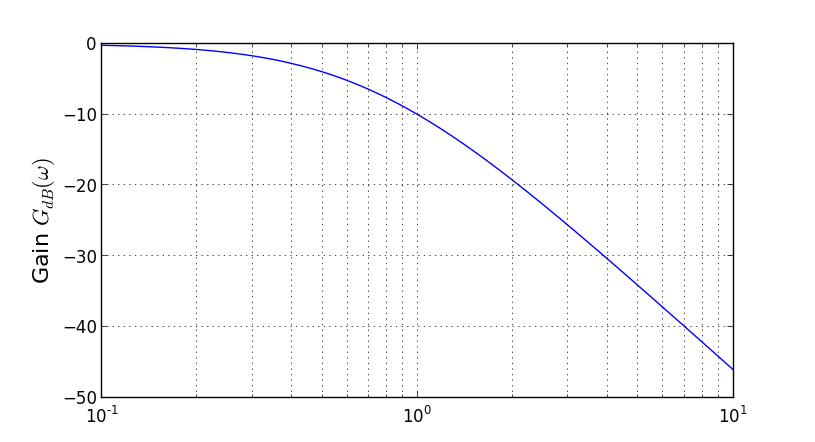
\includegraphics[scale=0.5]{figure_3.png} 
\end{center}
\legend {Fig. 3 : Filtre passe-bas passif non résonant}
\end{figure}

\begin{tBox}
\textbf{Question 6.} Écrire la fonction \texttt{pulsationCoupure(w,gain)} retournant la valeur de la pulsation de coupure \texttt{wc} en utilisant une méthode par balayage de la liste \texttt{gain}. On s'assurera de la terminaison de l'algorithme. Si la pulsation de coupure n'existe pas, on retourne -1.
\end{tBox}

\begin{dBox}
La méthode de dichotomie pour résoudre une équation est basée sur le théorème des valeurs intermédiaires. Soit $f : [a,b] \to \mathbb{R}$ une fonction continue, alors $f$ prend toutes les valeurs intermédiaires entre $f(a)$ et $f(b)$.
En particulier, si $f$ est telle que $f(a) \times f(b)<0$, alors il existe $\alpha \in ]a,b[$ tel que $f(\alpha) = 0$.
\end{dBox}

\begin{tBox} 
\textbf{Question 7.} Proposer une fonction \texttt{pulsationCoupure(w,gain)} retournant la valeur de la pulsation de coupure \texttt{wc} en utilisant une méthode de dichotomie sur la liste \texttt{gain}. Si la pulsation de coupure n'existe pas, on retourne -1.
\end{tBox}


\begin{tBox} 
\textbf{Question 8.}
\begin{enumerate}
\item Pour l'algorithme précédent, définir un variant de boucle et effectuer une preuve de terminaison,
\item Définir un invariant de boucle et effectuer une preuve de correction.
\item Quel intérêt présente la méthode de dichotomie par rapport à une méthode par balayage ?
\end{enumerate}
\end{tBox}

\vfill

\section{Stockage des données dans un fichier texte}

On souhaite stocker le contenu des listes \texttt{w}, \texttt{gain} et \texttt{phase} dans un fichier texte \texttt{"bode.txt"}.

L'annexe 2 donne quelques fonctions python.
Par exemple, pour ouvrir un fichier en écriture, on peut écrire \texttt{f = open("bode.txt","w")}. La variable \texttt{f} est alors un objet de type fichier.

La structure attendu dans le fichier texte \texttt{"bode.txt"} est la suivante (cas de la figure 2) :

\begin{dBox}
\hspace{0.5 cm} \texttt{pulsation;gain;phase}

\texttt{0.1;0.290546581842;-0.306830090606}

\texttt{0.12;0.421009962397;-0.373102215459}

\texttt{0.14;0.577344844946;-0.442256557908}

\texttt{...}
\end{dBox}

\begin{remark}
La première ligne permet de préciser le type des données du fichier.
La suite comporte autant de lignes que de données. Les séparateurs sont des points virgules ";".
\end{remark}

\begin{tBox}
\textbf{Question 9.}
\begin{enumerate}
\item Quelle sera la taille approximative du fichier texte \texttt{"bode.txt"} sachant que le nombre de données est identique à celui de la question 2 ?
\item Quel serait le gain de taille en \% si on se limitait à 3 chiffres significatifs pour chacune des valeurs numériques ?
\end{enumerate}
\end{tBox}

\begin{tBox}
\textbf{Question 10.} Écrire un script utilisant les listes \texttt{w}, \texttt{gain} et \texttt{phase}, et permettant de créer le fichier "bode.txt". A la fin de l'écriture, on assurera sa fermeture "propre".
\end{tBox}

\begin{tBox}
\textbf{Question 11.} Proposer une fonction \texttt{retourneListes(nomFichier)} prenant en argument une chaîne de caractère \texttt{nomFichier} et retournant les listes \texttt{w} (pulsations) et \texttt{gain} (gains). A la fin de la lecture, on assurera la fermeture "propre" du fichier.
\end{tBox}

\vspace{3 cm}

\begin{center}
- Fin de sujet -
\end{center}

\vfill


\pagebreak
\begin{center}
\huge{Annexe 1 : Diagrammes de Bode}
\end{center}
\lstinputlisting[language=Python,firstnumber=1,numbers=left]{Algorithmes/bode.py}

\vfill

\pagebreak
\begin{center}
\huge{Annexe 2 : Fonctions Python}
\end{center}

\begin{center}
--------- types ---------
\end{center}


\textsf{\textbf{str(x):}} Return a string version of the x object. If object is not provided, returns the empty string.

\vspace{.5cm}

\textsf{\textbf{int(x, base=10):}} Convert a number or string x to an integer, or return 0 if no arguments are given. If x is a number, return x.\_\_int\_\_(). For floating point numbers, this truncates towards zero.

If x is not a number or if base is given, then x must be a string, bytes, or bytearray instance representing an integer literal in radix base.

\vspace{.5cm}

\textsf{\textbf{float(x):}} Return a floating point number constructed from a number or string x.

If the argument is a string, it should contain a decimal number, optionally preceded by a sign, and optionally embedded in whitespace. The optional sign may be '+' or '-'; a '+' sign has no effect on the value produced.

\begin{center}
--------- fichiers ---------
\end{center}

\textsf{\textbf{open(file, mode='r', buffering=-1, encoding=None, errors=None, newline=None,
closefd=True, opener=None):}} Open file and return a corresponding file object. If the file
cannot be opened, an OSError is raised.

file is either a string or bytes object giving the pathname.

mode is an optional string that specifies the mode in which the file is opened. It defaults
to 'r' which means open for reading in text mode. Other common values are 'w' for writing
(truncating the file if it already exists), 'x' for exclusive creation and 'a' for appending (which
on some Unix systems, means that all writes append to the end of the file regardless of the
current seek position).

\vspace{.5cm}

\textsf{\textbf{close():}} Flush and close this stream. This method has no effect if the file is already closed.
Once the file is closed, any operation on the file (e.g. reading or writing) will raise a ValueError.
As a convenience, it is allowed to call this method more than once ; only the first call, however,
will have an effect.

\vspace{.5cm}

\textsf{\textbf{readline(size=-1):}} Read until newline or EOF and return a single str. If the stream is already at EOF, an empty string is returned.
If size is specified, at most size characters will be read.

\vspace{.5cm}

\textsf{\textbf{write(s):}} Write the string s to the stream and return the number of characters written.

\begin{center}
--------- chaînes de caractères ---------
\end{center}

\textsf{\textbf{split(str=" "):}} Method that returns a list of all the words in the string, using str as the separator (splits on all whitespace if left unspecified), optionally limiting the number of splits to num.

\begin{center}
--------- bibliothèque numpy ---------
\end{center}

Fonctions mathématiques : \textsf{\textbf{log(x)}}, \textsf{\textbf{exp(x)}}, \textsf{\textbf{cos(x)}}, \textsf{\textbf{sin(x)}}, etc.


\end{document}
